\chapter{Modell zur Integration von Erklärungen}

Das folgende Kapitel beschreibt das Modell für Erklärbarkeit, welches auf Basis der vorangegangenen Literaturrecherche entwickelt wurde (Siehe \autoref{sec:literature_review}). Zuerst werden die konkreten Anforderungen vorgestellt, welche in vorangegangener Literatur erarbeitet wurden, die für ein Modell für Erklärbarkeit gelten sollten. Neben einem Überblick über die verschiedenen Gesichtspunkte, die bei der Entwicklung von Erklärungen in einem erklärbaren System betrachtet werden sollten (\autoref{sec:model_overview}), werden in \autoref{sec:model_explanation_aspects} außerdem Ausprägungen für die Kategorien des Modells aufgezeigt, die in der Literatur bereits Anwendung gefunden haben. \autoref{sec:model_proved_relations} enthält eine Übersicht von bereits gezeigten Zusammenhängen zwischen bestimmten Aspekten von Erklärungen basierend auf der Zusammenfassung der verschiedenen Aspekte von Erklärbarkeit. Abschließend werden in diesem Kapitel die Auswirkungen daraus für das Design von Erklärungen vorgestellt (\autoref{sec:model_design_implications}).

\section{Anforderungen}

Nach einer Untersuchung von Erklärungen stellen mehrere Autoren den Bedarf für eine Vereinheitlichung der Untersuchung von Erklärungen fest \cite{cirqueira_scenario-based_2020,zahedi_towards_2019, nunes_systematic_2017, martin_evaluating_2021}. Dies soll es ermöglichen, den Vergleich zwischen verschiedenen Lösungsansätzen zu vereinfachen. In einigen Arbeiten fordern die Autoren, dass ein einheitliches Framework zur Evaluation benötigt wird, anhand dessen die Qualität von Erklärungen bestimmt werden kann \cite{nunes_systematic_2017,sokol_explainability_2020,chari_explanation_2020}. Allerdings wird auch darauf verwiesen, dass es einer Unterstützung bedarf, um Anforderungen an die Erklärungen zu formulieren bzw. die Probleme, welche durch Erklärungen gelöst werden sollen zu identifizieren \cite{chazette_end-users_nodate, doshi2017towards}. Unterstützt wird dies durch \citeauthor{waa_evaluating_2021}, welche dies nutzen wollen, um jeder Prüfung von Erklärungen klare Hypothesen voraus zustellen, um die Ergebnisse verschiedener Arbeiten besser zusammenfassen und daraus Empfehlungen ableiten zu können. Auch \citeauthor{kohl_explainability_2019} unterstreicht den Aspekt, dass vor allem die Ziele und Anforderungen auf Basis des aktuellen Kontextes klar sein müssen, bevor Erklärungen in ein System integriert werden. Folglich sollte das Modell auch hierfür Unterstützung bieten. Außerdem ergibt sich aus dem Ziel der Arbeit (\autoref{sec:goal_definition}), dass das Modell auch Gestaltungsempfehlungen für Erklärungen enthalten und somit einen Teil der Forderung von \citeauthor{waa_evaluating_2021} nach einem Überblick über bisherige Ergebnisse erfüllen soll. Basis hierfür sind die Forschungsfragen RQ2 und RQ3, welche nach den Auswirkungen verschiedener Eigenschaften von Erklärungen fragen. Voraussetzung dafür ist allerdings auch, dass mögliche Eigenschaften von Erklärungen definiert werden (RQ1).

Zusammenfassend kann man also sagen, dass dieses Modell vor allem drei Aspekte erfüllen muss:

\begin{enumerate}
    \item Das Modell muss das Erheben von Anforderungen an Erklärungen und das Aufstellen von Hypothesen über den Einfluss vereinfachen.
    \item Im Modell sollten die bereits evaluierten möglichen Formen von Erklärungen dargestellt werden.
    \item Das Modell muss einen Überblick über verschiedene Evaluationsmöglichkeiten geben, um die Qualität von integrierten Erklärungen im Nachhinein zu bewerten.
    \item Es müssen existente Ergebnisse aus der Literatur so im Modell zusammengefasst sein, dass es für einen Nutzer des Modells möglich ist, diese auf seinen Kontext zu übertragen und folglich Erklärungen in ein System zu integrieren.
\end{enumerate}

\section{Modellübersicht}

\begin{itemize}
    \item Qualitätsmodelle \cite{schneider2012abenteuer}
    \item GQM \cite{briand1995goal, schneider2012abenteuer} needs enviromental characteristics and product information (kontext), auch gezeigt in der Definition von Erklärbarkeit durch \cite{chazette_knowledge_nodate}.
    \item zentraler aspekt von \cite{briand1995goal} ist außerdem 
    \item Außerdem werden existierende Konzepte und Abstraktionen benötigt \cite{briand1995goal}. Diese werden bereits in vielen Arbeiten vorgestellt, wie die Literaturrecherche gezeigt hat. (siehe section...)
    \item final muss 
\end{itemize}

Um RQ1 und 2 definieren zu können

Welche Äußeren Einflüsse Auswirkungen auf eine Erklärung haben.

Erstes Level der Abstraktion für Erklärungen:

\begin{itemize}
    \item In welchem Kontext soll sie angezeigt werden? \cite{kohl_explainability_2019, chazette_knowledge_nodate}
    \item Warum sollte sie angezeigt werden (mit welchem Ziel)? \cite{kohl_explainability_2019, rosenfeld_explainability_2019}
    \item Was sollte wann und wie angezeigt werden (Was sind die Charakteristiken der Erkärung)? \cite{kohl_explainability_2019, rosenfeld_explainability_2019}
\end{itemize}

Alle expliziten Erwähnungen von diesen Oberbegriffen in \autoref{tab:model_explaination_aspects}. Um die Schritte beim integrieren vom erklären klar zu machen, habe ich die Oberkategorien, die von 

\cite{rosenfeld_explainability_2019} stellt die Fragen:.... Ebenfalls unterstützt in \cite{chazette2020explainability}

\cite{rosenfeld_explainability_2019} sagen, dass zu erst die die Ziele einer Erklärung betrachtet werden sollen (\glqq \textit{Warum} benötigt das System eine Erklärung? \grqq{}) vgl. Seite 699 \cite{rosenfeld_explainability_2019}. \cite{cirqueira_scenario-based_2020} sagen, dass über haupt erst einmal der Kontext (\glqq Stakeholder Setting\grqq{}) klar werden muss.

\begin{longtable}{|p{.2\textwidth}|p{.5\textwidth}|p{.2\textwidth}|}
    \hline
    \textbf{Aspekt}          & \textbf{Synonyme} & \textbf{Quellen} \\ \hline
    Context         & (Experimental) Context & \cite{chazette_knowledge_nodate} \cite{chazette_end-users_nodate} \cite{sato_context_nodate} \cite{waa_evaluating_2021} \cite{kohl_explainability_2019} \cite{neerincx_using_2018} \cite{sovrano_modelling_2020} \cite{doshi2017towards} \\
                    & (Explanation) Scope & \cite{wohlin2012experimentation} \cite{eiband_impact_2019} \cite{doshi2017towards} \\
                    & Use Case & \cite{waa_evaluating_2021} \\
                    & Who & \cite{rosenfeld_explainability_2019} \\
    \hline
    Objective       & Objective & \cite{nunes_systematic_2017} \\
                    & Construct & \cite{waa_evaluating_2021} \\
                    & Purpose & \cite{nunes_systematic_2017} \cite{wohlin2012experimentation} \\
                    & (Stakeholder) Goals & \cite{cirqueira_scenario-based_2020} \cite{sovrano_modelling_2020} \cite{ribera2019can} \\
                    & Main Drive & \cite{anjomshoae2019explainable} \\
                    & Intended Effect & \cite{balog_measuring_2020} \\
    \hline
    Characteristics & Aspects       & \cite{rosenfeld_explainability_2019} \\
                    & User Interface Component(s) & \cite{nunes_systematic_2017} \cite{rosenfeld_explainability_2019} \\
                    & What? How? When? & \cite{rosenfeld_explainability_2019} \\
                    & Content and Type & \cite{ribera2019can} \\
    \hline
    Evaluation      & Evaluation    & \cite{kohl_explainability_2019} \cite{doshi2017towards} \\
                    & Measurements  & \cite{waa_evaluating_2021} \cite{balog_measuring_2020} \\
                    & Metrics       & \cite{nunes_systematic_2017} \cite{anjomshoae2019explainable} \cite{chari_explanation_2020} \cite{waa_evaluating_2021}\\
    \hline
\caption{Allgemeine Aspekte von Erklärungen in der Literatur}
\label{tab:model_explaination_aspects}
\end{longtable}

Außerdem muss, nach dem Kontext und die Ziele klar sind die Frage beantwortet werden welcher Explanda X überhaupt erklärt werden sollen \cite{kohl_explainability_2019}

\section{Aspekte von Erklärungen}
\label{sec:model_explanation_aspects}

Literatur, die einen Überblick über Erklärbarkeit im Allgemeinen oder in einem bestimmten Anwendungsfeld gibt, betrachtet in der Regel fünf Aspekte von Erklärbarkeit \cite{rosenfeld_explainability_2019, nunes_systematic_2017,chazette_knowledge_nodate}. Dies sind der Kontext der Erklärung, die Zielsetzung dieser, welche Erklärung angezeigt werden soll und wann diese angezeigt werden soll. In einigen Arbeiten wird bei der angezeigten Erklärung außerdem zwischen dem Inhalt und der Darstellung unterschieden bzw. diese Eigenschaften einzeln untersucht \cite{nunes_systematic_2017,abdulrahman_belief-based_2019}. Darüber hinaus wird in allen hier betrachteten Arbeiten auch die Evaluation von Erklärungen thematisiert (Siehe \autoref{sec:literature_review}).

Für die zuvor genannten Aspekte werden in der Literatur verschiedene Unterkategorien konkret benannt oder Synonyme verwendet. \autoref{tab:model_explaination_aspects} fasst die verwendeten Synonyme aus den Veröffentlichungen, welche den Aspekt explizit erwähnt haben, unter der final gewählten Benennung zusammen. Neben den dort aufgezeigten Begriffen haben mehrere Autoren (z.~B. \cite{rosenfeld_explainability_2019, chazette2020explainability}) die verschiedenen Aspekte von Erklärbarkeit zusätzlich mit Fragewörtern verknüpft. Die vollständigen Fragen dahinter verweisen allerdings auf verschiedene Unterpunkte, weswegen das vorgestellte Modell auf Fragewörter verzichtet, um Verwechselungen vorzubeugen. (Beispiel: \glqq \textbf{Wie} kann die Erklärung evaluiert werden?\grqq{} (\textit{Evaluation}) \cite[vgl.][]{rosenfeld_explainability_2019} und \glqq \textbf{Wie} viele Informationen sollte jede Erklärung enthalten?\grqq{} (\textit{Content}) \cite[vgl.][]{kouki_user_2017}).

\bigskip

Im Folgenden werden die genannten Oberkategorien erläutert bzw. definiert.

\begin{table}
    \begin{tabular}{|p{.2\textwidth}|p{.4\textwidth}|p{.3\textwidth}|}
        \hline
        \textbf{Aspekt} & \textbf{Synonyme}         & \textbf{Quellen} \\ \hline
        1. Context      & (Experimental) Context    & \cite{chazette_knowledge_nodate} \cite{chazette_end-users_nodate}
                                                    \cite{sato_context_nodate} \cite{waa_evaluating_2021} 
                                                    \cite{kohl_explainability_2019} \cite{neerincx_using_2018} 
                                                    \cite{sovrano_modelling_2020} \cite{doshi2017towards} \\
                        & (Explanation) Scope       & \cite{wohlin2012experimentation} \cite{eiband_impact_2019}
                                                    \cite{doshi2017towards} \\
                        & Use Case                  & \cite{waa_evaluating_2021} \\
                        & Stakeholder               & \cite{rosenfeld_explainability_2019} \\
        \hline
        2. Objectives   & Objectives                & \cite{nunes_systematic_2017} \\
                        & Construct                 & \cite{waa_evaluating_2021} \\
                        & Purpose                   & \cite{nunes_systematic_2017} \cite{wohlin2012experimentation} \\
                        & (Stakeholder) Goals       & \cite{cirqueira_scenario-based_2020}
                                                    \cite{sovrano_modelling_2020} \cite{ribera2019can} \\
                        & Main Drive                & \cite{anjomshoae2019explainable} \\
                        & Intended Effect           & \cite{balog_measuring_2020} \\
        \hline
        3. Demand       & Demand                    & \cite{chazette_knowledge_nodate} \\
        \hline
        4. Content      & User Interface Component(s) & \cite{nunes_systematic_2017}
                                                    \cite{rosenfeld_explainability_2019} \\
                        & Content                   & \cite{ribera2019can} \\
                        & Granularity               & \cite{chazette_knowledge_nodate}
                                                    \cite{kohl_explainability_2019} \\
        \hline
        5. Presentation & Presentation              & \cite{rosenfeld_explainability_2019} \cite{kouki_user_2017} \\
                        & (Explanation) Type        & \cite{ribera2019can} \cite{rosenfeld_explainability_2019} \\
        \hline
        6. Evaluation   & Evaluation                & \cite{kohl_explainability_2019} \cite{doshi2017towards} \\
                        & Measurements              & \cite{waa_evaluating_2021} \cite{balog_measuring_2020} \\
                        & Metrics                   & \cite{nunes_systematic_2017} \cite{anjomshoae2019explainable}
                                                    \cite{chari_explanation_2020} \cite{waa_evaluating_2021}\\
        \hline
    \end{tabular}
\caption{Übergeordnete Aspekte von Erklärungen in der Literatur}
\label{tab:model_explaination_aspects}
\end{table}

\paragraph{Context} Der \textit{Context} einer Erklärung wird durch die Situation gegeben, welche durch die Interaktion eines Nutzers, seiner Aufgabe, dem System und der Umgebung entsteht. (\cite[vgl.][]{chazette_knowledge_nodate, kohl_explainability_2019}).

\paragraph{Objectives} \textit{Objectives} sind die Qualitätsziele, welche für eine Erklärung gelten oder aufgrund derer Erklärungen in ein System integriert werden sollen.

\paragraph{Demand} Der \textit{Demand} für eine Erklärung ist der Bedarf für Erklärungen durch den Nutzer eines Systems. Das heißt der \textit{Demand} beschreibt die Notwendigkeit, zu einemen bestimmten Zeitpunkt für einen Systemteil Erklärungen bereitzustellen. Das beinhaltet auch, ob die Initiative vom Nutzer ausgeht oder das System selbstständig eine Erklärung anzeigt.

\paragraph{Content} Der \textit{Content} einer bei bestehendem Bedarf dem Nutzer bereitgestellten Erklärung ist durch die Informationen und die Informationsdichte definiert.

\paragraph{Presentation} Der Inhalt einer Erklärung kann Nutzern auf verschiedenen Wegen zugänglich gemacht werden. Die \textit{Presentation} einer Erklärung ist die Art und Weise, auf die dem Nutzer die Informationen durch die Erklörung bereitgestellt werden.

\paragraph{Evaluation} Die \textit{Evaluation} ist die Bewertung der Qualität von Erklärungen. Dies enthält die grundsätzlichen verschiedenen Evaluationsmöglihckeiten und- Metriken mit denen die Qualität gemessen werden kann.

\subsection{Struktur des Modells}

Die Struktur des Modells für Erklärungen orientiert sich an den Forschungsfragen und Anforderungen an das Modell, Ergebnissen aus der Literaturrecherche sowie dem bestehenden Konzept der Qualitätsmodelle \cite{schneider2012abenteuer} (Siehe \autoref{sec:basics_quality_models}).

In der Literatur wurden einige Aspekte des Modells nicht nur verschieden genannt, sondern auch zum Teil in Oberkategorien gegliedert oder auf verschiedenen Abstraktionsebenen betrachtet. Hieraus ergibt sich eine Hierarchische Anordung des Modells. Verschiedene Abstraktionsebenen enthalten auch die von \citeauthor{schneider2012abenteuer} vorgestellten Qualitätsmodelle \cite{schneider2012abenteuer}. Dabei werden abstrakte Ziele (\textit{Objectives}) immer weiter konkretisiert, bis sie schlussendlich mit konkreten Metriken messbar sind. Das zugrunde liegende Modell (\glqq Goal-Driven and Property-Based Definition Approach for Product Metrics\grqq{} \cite{briand1995goal}) von \citeauthor{briand1995goal} definiert außerdem unter anderem die nötigen Abhängigkeiten der \textit{Objectives} von äußeren Faktoren, die im hier vorgestellten Modell für Erklärungen dem bereits erwähnten \textit{Context} entsprechen.

Die Betrachtung von \textit{Context} und \textit{Objectives} erfolgt in der Literaur über Erklärungen zum Teil in verschiedener Reihenfolge. \citeauthor{rosenfeld_explainability_2019} schreiben, dass die erste Frage, welche geklärt werden sollte, die Frage \glqq Warum benötigt das System eine Erklärung?\grqq{} ist \cite[vgl. S. 699][]{rosenfeld_explainability_2019}\cite{nunes_systematic_2017}. Im Gegensatz dazu schreiben \citeauthor{cirqueira_scenario-based_2020}, dass zuerst äußere Umstände, wie der Endnutzer des Systems geklärt sein sollte (\glqq Stakeholder Setting\grqq{} \cite{cirqueira_scenario-based_2020}), um darauf aufbauend die Ziele festzulegen. Hieraus wird geschlussfolgert, dass die Festlegung der Ziele mit ihren Abhängigkeiten wie auch von \cite{schneider2012abenteuer} geschildert eine iterative, stark zusammenhängende Aufgabe ist. Daher werden die Punkte \textit{Context} und \textit{Objectives} aus \autoref{tab:model_explaination_aspects} unter \textit{External Dependencies} zusammengefasst. Dies verdeutlicht, dass die \textit{Objectives} für das Integrieren von Erklärungen stark mit anderen äußeren Einflüssen (\textit{Context}) zusammenhängen (\autoref{sec:model_external_dependencies}).

Auch werden \textit{Demand}, \textit{Content} und \textit{Presentation} vereint dargestellt, da sich diese drei Kategorien direkt auf die Eigenschaften von Erklärungen beziehen (\textit{Characteristics}). Damit wird der Zusammenhang zwischen den verschiedenen Merkmalen einer Erklärung verdeutlicht \cite{nunes_systematic_2017}.

Zusätzlich zur Zielevaluation von Qualitätsmodellen betrachtet das vorgestellte Modell die unmittelbare Evaluation von Erklärungen. Diese müssen einzeln betrachtet werden, da für diese die Metriken zum Teil erst nach der Entwicklung der Erklärungen festgelegt werden können.

\smallbreak

Schlussendlich ist das Modell in die drei Oberkategorien \textit{External Dependencies}, \textit{Characteristics} und \textit{Evaluation} gegliedert. Eine Übersicht ist in \autoref{fig:model_overview} zu sehen. Die Gesamtübersicht des Modells für Erklärungen bietet \autoref{fig:model_overview_complete}. Diese enthält darüber hinaus die in den folgenden Abschnitten beschriebenen Ausprägungen der einzelnen Kategorien aus der Literatur. Die Gesamtübersicht ist grafisch an der Taxonomie für Erklärungen von \citeauthor{nunes_systematic_2017} angelehnt und enthält auch einige Aspekte daraus \cite{nunes_systematic_2017}. Die erwähnte Taxonomie ist allerdings nur auf den Einsatz von Erklärungen in Empfehlungssystemen bezogen und beschränkt sich daher u.~a. auf bestimmte Darstellungstypen. Sie kann folglich nicht ohne Weiteres in andere Kontexte übertragen werden. Darüber hinaus fehlt der Aspekt der Evaluation. Dieser wird allerdings nicht nur von \citeauthor{nunes_systematic_2017} selbst, sondern auch von weiteren Autoren für wichtig erachtet \cite{cirqueira_scenario-based_2020, martin_evaluating_2021}.

\begin{figure}[htb!]
    \begin{center}
        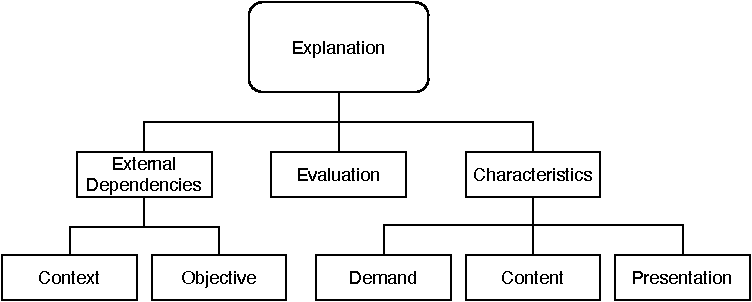
\includegraphics[width=0.9\linewidth]{contents/05_model_description/res/model-overview.pdf}
    \end{center}
    \caption{Oberkategorien der Aspekte von Erklärungen}
    \label{fig:model_overview}
\end{figure}

\subsection{Externe Abhängigkeiten}
\label{sec:model_external_dependencies}

Unter \textit{External Dependencies} sind die Aspekte zusammengefasst, die eine Auswirkung auf Erklärungen in einem System haben. Außerdem können von den hier aufgeführten Punkten Anforderungen abgeleitet und später zusammen mit Metriken Hypothesen aufgestellt werden. Daraus kann dann auch abgeleitet werden, welche Funktionen des Systems einer Erklärung bedürfen \cite{kohl_explainability_2019}.

Wie bereits beschrieben, sind die \textit{External Dependencies} in den \textit{Context} und die \textit{Objectives} unterteilt. Über die Reihenfolge, in der ein Stakeholder, der Erklärungen in ein System integrieren möchte, die beiden Aspekte betrachten sollte, gibt es in der Literatur unterschiedliche Meinungen. \citeauthor{rosenfeld_explainability_2019} schreiben, dass die erste Frage, welche geklärt werden sollte, die Frage \glqq Warum benötigt das System eine Erklärung?\grqq{} ist \cite[vgl. S. 699][]{rosenfeld_explainability_2019}. Im Gegensatz dazu schrieben \citeauthor{cirqueira_scenario-based_2020}, dass zuerst äußere Umstände, wie der Endnutzer des Systems geklärt sein sollte (\glqq Stakeholder Setting\grqq{} \cite{cirqueira_scenario-based_2020}), um darauf aufbauend die Ziele festzulegen. Laut \citeauthor{briand1995goal} hat zumindest auf die Ziele einer Evaluation der Kontext des Systems einen Einfluss und sollte somit zuvor geklärt werden \cite{briand1995goal}. Aus den verschiedenen Ansichten wird gefolgert, dass der \textit{Context} des Systems und die \textit{Objectives} eng zusammen hängen und nur gemeinsam betrachtet werdeb können.

\subsubsection{Context}

Der \textit{Context} einer Erklärung beschreibt die äußeren Einflüsse, die unmittelbar auf das erklärbare System wirken und somit Anforderungen an die Eigenschaften von Erklärungen stellen.

Dies beinhaltet die Aktivität, die der Endbenutzer in einer bestimmten Umgebung durchführt. Aus den Eigenschaften der drei genannten Aspekte leiten sich dabei direkte Einflüsse auf den Bedarf, den Inhalt und die Darstellung einer Erklärung ab.

In der

Der Begriff Stakeholder wurde hier verschieden eingesetzt. Beispielsweise nutzen \citeauthor{cirqueira_scenario-based_2020}den Begriff für den Nutzer einer Software \cite{cirqueira_scenario-based_2020} und \cite{nunes_systematic_2017} als Oberbegriff für Personengruppen, die ein Interesse an einem System haben, den Nutzer allerdings ausschließen \cite{nunes_systematic_2017}. Diese Arbeit geht von der Definition nach (Quelle suchen) aus, welch alle interessieren Gruppen beschreibt. 

Das Modell von \cite{nunes_systematic_2017} enthält allerdings weder den Kontext noch den Evaluationspart, welcher für einen Überblick über Erklärbarkeit wichtig ist. Der Fokus ist eher auch auf Recommender Systems gelegt

Nur die Kontexte, die explizit erwähnt wurden in \autoref{tab:impact_of_context_on_explanation}

\begin{table}
    \begin{tabular}{|p{.2\textwidth}|p{.5\textwidth}|p{.2\textwidth}|}
        \hline
        \textbf{Aspekt} & \textbf{Synonyme} & \textbf{Quellen} \\ \hline
        End User        &  (Targt / End)  User & \cite{chazette2020explainability} \cite{kaptein_personalised_2017} \cite{sokol_one_2020} \cite{wiegand_id_2020} \\
                        & Stakeholder & \cite{chazette_knowledge_nodate} \\
                        & Consumer & \cite{ehsan_human-centered_2020} \\
                        & Explainee & \cite{chazette_knowledge_nodate} \cite{kohl_explainability_2019} \\
        \hline
        Environment     & Environment & \cite{chazette_knowledge_nodate} \cite{wiegand_id_2020} \cite{wiegand2019drive} \\
                        & Application Area & \cite{sokol_explainability_2020} \cite{wiegand2019drive} \cite{wiegand_id_2020} \\
        \hline
        Task            & Task & \cite{chazette_knowledge_nodate} \cite{sokol_explainability_2020} \cite{gunning2019darpa} \\
                        & Activity & \cite{wohlin2012experimentation} \\
                        
        \hline
    \end{tabular}
    \caption{Kontext einer Erklärung}
    \label{tab:impact_of_context_on_explanation}
\end{table}

\paragraph{Endnutzer}

Different synonyms for it like....

\paragraph{Äußere Bedingungen}

\paragraph{Aufgabe}

\subsubsection{Zielsetzung}
\label{subsec:model_objective}

\cite{chazette_knowledge_nodate} haben einen Katalog zusammengestellt, der die Einflüsse von Erklärbarkeit darstellt

\cite{tintarev_designing_nodate} haben Messliste gebaut.

Nur Erwähnung, wenn das Paper den Aspekt explizit untersucht / erwähnt. In \autoref{tab:quality_aspects_of_explanation} sind alle Arbeiten aufgelistet, die Erklärbarkeit entweder im Bezug auf den aufgelisteten Qualitätsaspekt untersuchen oder 

\begin{table}
    \begin{center}
        \begin{tabular}{|p{.24\textwidth}|p{.5\textwidth}|p{.2\textwidth}|}
            \hline
            \textbf{Qualitätsaspekt}    & \textbf{Beschreibung} & \textbf{Quellen} \\ \hline
            Transparency                & Erklärung, wie das System funktioniert.
                                        & \cite{nunes_systematic_2017} \cite{chazette_knowledge_nodate} \cite{tintarev_designing_nodate} \cite{chazette_end-users_nodate} \cite{balog_measuring_2020} \cite{chazette2020explainability} \cite{tintarev2015explaining} \cite{hernandez-bocanegra_effects_2020} \cite{tsai_effects_2020} \cite{rjoob_towards_2021}  \cite{sokol_one_2020} \cite{wang_is_2018} \cite{koo_understanding_2016} \cite{tintarev2007survey}\\ \hline
            Understandability           & ggf. löschen, da Transparency SIG / Mental Model
                                        & \cite{chazette_knowledge_nodate} \cite{chazette_end-users_nodate} \cite{martin_evaluating_2021}  \cite{ehsan_human-centered_2020} \cite{rjoob_towards_2021}  \cite{sokol_one_2020} \cite{cheng2019explaining} \\ \hline
            Trust                       & Das Vertrauen des Nutzers in das System erhöhen.
                                        & \cite{nunes_systematic_2017} \cite{chazette_knowledge_nodate} \cite{tintarev_designing_nodate} \cite{balog_measuring_2020} \cite{eiband_impact_2019} \cite{tintarev2015explaining} \cite{hernandez-bocanegra_effects_2020} \cite{stange_effects_2021} \cite{weitz_you_2019} \cite{yamada_evaluating_2016} \cite{haspiel_explanations_2018} \cite{martin_developing_2019} \cite{martin_evaluating_2021} \cite{tsai_effects_2020}  \cite{sokol_one_2020}  \cite{wang_is_2018} \cite{koo_understanding_2016} \cite{wiegand2019drive} \cite{gunning2019darpa} \cite{lim_2009_assessing} \cite{tintarev2007survey} \cite{kunkel_let_2019} \\ \hline
            Satisfaction                & Benutzerfreundlichkeit und generelle Zufriedenheit mit dem System erhöhen.
                                        & \cite{nunes_systematic_2017} \cite{chazette_knowledge_nodate} \cite{tintarev_designing_nodate} \cite{balog_measuring_2020} \cite{tsai_evaluating_2019} \cite{tintarev2015explaining} \cite{riveiro_thats_2021} \cite{martin_developing_2019} \cite{martin_evaluating_2021} \cite{tsai_effects_2020} \cite{ehsan_human-centered_2020} \cite{sovrano_modelling_2020} \cite{koo_understanding_2016} \cite{ribera2019can} \cite{gunning2019darpa} \cite{lim_2009_assessing}  \cite{tintarev2007survey} \cite{sato_context_nodate} \\ \hline
            Scrutability                & Dem Nutzer die Möglichkeit geben, dem System einen Fehler mitzuteilen 
                                        & \cite{nunes_systematic_2017} \cite{chazette_knowledge_nodate} \cite{tintarev_designing_nodate} \cite{balog_measuring_2020} \cite{tintarev2015explaining} \cite{martin_developing_2019} \cite{gunning2019darpa}  \cite{tintarev2007survey} \cite{martin_evaluating_2021} \\ \hline
            Efficiency                  & Das Verhältnis von Qualität und Zeit für das Lösen einer Aufgabe verbessern.
                                        & \cite{nunes_systematic_2017} \cite{chazette_knowledge_nodate} \cite{tintarev_designing_nodate} \cite{balog_measuring_2020} \cite{tsai_evaluating_2019} \cite{tintarev2015explaining} \cite{hernandez-bocanegra_effects_2020} \cite{tintarev2007survey}\\ \hline
            Effectiveness               & Die Qualität der Aufgabe des Nutzers erhöhen
                                        & \cite{nunes_systematic_2017} \cite{chazette_knowledge_nodate} \cite{tintarev_designing_nodate} \cite{balog_measuring_2020} \cite{tintarev2015explaining} \cite{zolotas_towards_2019} \cite{hernandez-bocanegra_effects_2020} \cite{martin_evaluating_2021} \cite{rjoob_towards_2021} \cite{tintarev2007survey} \\ \hline
            Persuasiveness              & Convince Users to try or by. \cite{balog_measuring_2020}
                                        & \cite{nunes_systematic_2017} \cite{tintarev_designing_nodate} \cite{balog_measuring_2020} \cite{sato_context_nodate} \cite{sato_context_nodate} \cite{abdulrahman_belief-based_2019} \cite{tintarev2015explaining} \cite{sato_action-triggering_2019} \cite{tintarev2007survey} \\ \hline
        \end{tabular}
    \end{center}
    \caption{Qualitätsaspekte einer Erklärung}
    \label{tab:quality_aspects_of_explanation}
\end{table}

1. To justify its decisions so the human participant can decide to accept them (provide control) 2. To explain the agent’s choices to guarantee safety concerns are met 3. To build trust in the agent’s choices, especially if a mistake is suspected or the human operator does not have experience with the system 4. To explain the agent’s choices to ensure fair, ethical, and/or legal decisions are made 5. Knowledge/scientific discovery 6. To explain the agent’s choices to better evaluate or debug the system in previously unconsidered situations \cite{rosenfeld_explainability_2019}

Usability beschreibt die Qualität einer Erklärung im Bezug auf die Interaktion und die Darstellung Darstellung der Inhalte \cite{chazette_end-users_nodate}. Informativeness ist dierekt bezogen auf den Inhalt der Erklärung \cite{chazette_end-users_nodate}. Direkt messbar an der Erklärung selbst.

\cite{schneider2012abenteuer} beschreibt den Prozess von abstrakten allgemein definierten und bekannten Qualitätszielen hin zu konkreten Metriken. Als Zwischenstufe werden konkrete Qualitätsziele, die für den aktuellen Anwendungsfall gültig sind aufgestellt. \cite{nunes_systematic_2017} und \cite{waa_evaluating_2021} unterteilen diese verschiedenen Abstraktionsebenen der Ziele für Erklärungen in drei Ebenen. Die ursprünglichen Begrifflichkeiten der beiden erwähnten Arbeiten sowie weitere Synonyme aus anderen Arbeiten sind in \autoref{tab:impact_of_objective_on_explanation} zusammengefasst.

7 Established goals von \cite{tintarev2015explaining, tintarev_designing_nodate}

Einteilung in Oberkategorien...

\begin{longtable}{|p{.2\textwidth}|p{.5\textwidth}|p{.2\textwidth}|}
    \hline
    \textbf{Aspekt}     & \textbf{Synonym} & \textbf{Quellen} \\ \hline
    Business Goals      & Motivation & \cite{nunes_systematic_2017} \\
                        & Stakeholder Goals & \cite{nunes_systematic_2017} \\
                        & (Intended) Purpose & \cite{waa_evaluating_2021} \\
                        & Higher-level Goals & \cite{nunes_systematic_2017} \\
                        & Application Level & \cite{sokol_explainability_2020} \\
    \hline
    Users' Perception   & User Perceived Quality Factors & \cite{nunes_systematic_2017} \\
                        & (Consumer) Needs & \cite{ehsan_human-centered_2020} \cite{chazette_end-users_nodate} \\
                        & User Goals & \cite{ehsan_human-centered_2020} \\
                        & Intermediate Requirements & \cite{waa_evaluating_2021} \\
                        & Human level & \cite{sokol_explainability_2020} \\
                        
    \hline
    Explanation Purpose & Purpose & \cite{nunes_systematic_2017} \\
                        & Explanatory Goal & \cite{tintarev_designing_nodate} \cite{balog_measuring_2020} \\
                        & Function Level & \cite{sokol_explainability_2020} \\
    \hline
\caption{Zielsetzung einer Erklärung}
\label{tab:impact_of_objective_on_explanation}
\end{longtable}

Determine what what information should be conveyed to the user \cite{nunes_systematic_2017}

Nach IEEE[Bearbeiten | Quelltext bearbeiten]
Laut IEEE[1] kann das requirements engineering unterteilt werden in:

Anforderungserhebung (requirements elicitation),
Anforderungsanalyse (requirements analysis),
Anforderungsspezifikation (requirements specification) und
Anforderungsbewertung (requirements validation)
Diese Tätigkeiten überlappen einander und werden oft auch mehrfach – iterativ – durchgeführt.

\subsection{Eigenschaften}

Die \textit{Characteristics} umfassen jene Eigenschaften von Erklärungen, die einen Einfluss auf die externe Qualität eben dieser haben. Unter dem Aspekt sind die Möglichkeiten zusammengefasst, die bei der Ausgestaltung von Erklärungen bestehen. Gegliedert sind die Eigenschaften in den Bedarf der Erklärung (\textit{Demand}), die ausgelieferten Informationen (\textit{Content}) und die Bereitstellung (\textit{Presentation}). Diese drei Unterkategorien werden in den folgenden Abschnitten vorgestellt. Wichtig zu beachten ist, dass sich die vorgestellten Möglichkeiten nicht unbedingt ausschließen. Das heißt vor allem, dass nicht jede Erklärung genau eine Ausprägung eines Aspektes erfüllen muss, sondern auch neue oder zwischen zwei Möglichkeiten liegende Eigenschaften aufweisen kann. Darüber hinaus muss auch nicht zwangsweise für jede Eigenschaftskategorie eine Eigenschaft ausgewählt werden, da nicht alle Kategorien auf jeden Kontext zutreffen.

\begin{figure}[htb!]
    \begin{center}
        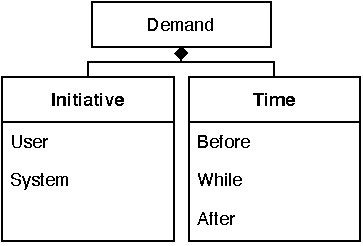
\includegraphics{contents/05_model_description/res/model_demand_overview.pdf}
    \end{center}
    \caption{Übersicht über den \textit{Demand} für Erklärungen}
    \label{fig:model_demand_overview}
\end{figure}

\subsubsection{Bedarf}

Der \textit{Demand}  für Erklärungen kann aus verschiedenen Perspektiven betrachtet werden. Bei welcher Aufgabe und bei welchen Ereignissen Erklärungen überhaupt benötigt werden, muss in den Anforderungen für Erklärungen festgehalten werden. Diese entstehen auf Basis der \textit{External Dependencies}. Unter der Kategorie \textit{Demand} in diesem Modell ist zusätzlich festgehalten, auf welche Initiative hin (\textit{Initiative}) und zu welchem Zeitpunkt in Bezug auf ein Ereignis im System dem \textit{End User} Erklärungen vom System zur Verfügung gestellt werden sollen. Einen Überblick über die Verwendung verschiedener Ausprägungen der Aspekte ist in \autoref{fig:model_demand_overview} und \autoref{tab:explanation_demands} dargestellt.

\begin{table}[bht!]
    \begin{center}
        \begin{tabular}{p{.25\textwidth}p{.25\textwidth}p{.41\textwidth}}
            \hline
            Aspekt    & Ausprägung   & Quellen \\
            \toprule
            Initiative  &  Manual       & \cite{chazette_end-users_nodate} \cite{tintarev_designing_nodate}
                                            \cite{wiegand_id_2020} \\
                        &  Automatic    & \cite{chazette_end-users_nodate} \cite{eiband_impact_2019}
                                            \cite{wiegand_id_2020} \cite{schaffer_i_2019}
                                            \cite{yamada_evaluating_2016} \\
            \tablerowspacing
            Time        &  Before       & \cite{rosenfeld_explainability_2019} \cite{wiegand_id_2020}
                                            \cite{kunkel_let_2019} \cite{koo_why_2015} \cite{haspiel_explanations_2018} 
                                            \cite{haspiel_explanations_2018} \\
                        &  while        & \cite{rosenfeld_explainability_2019} \cite{wiegand_id_2020}
                                            \cite{kunkel_let_2019} \\
                        &  After        & \cite{rosenfeld_explainability_2019} \cite{wiegand_id_2020}
                                            \cite{kunkel_let_2019} \cite{koo_why_2015} \cite{haspiel_explanations_2018}
                                            \cite{wiegand2019drive} \cite{haspiel_explanations_2018} \\
            \toprule
        \end{tabular}
    \end{center}
    \caption{Der Bedarf einer Erklärung zusammen mit in der Literatur untersuchten Einflüssen auf die Qualität von Erklärungen}
    \label{tab:explanation_demands}
\end{table}

\paragraph{Initiative} Die \textit{Initiative} einer Erklärung ist der Auslöser für das Geben von Erklärungen in einem System. Eine Möglichkeit ist eine automatische Auslieferung der Erklärung an den \textit{End User}. Das System trifft dann allein die Entscheidung, wann und ob \textit{End User} eine Erklärung bekommt (\textit{Automatic}). Alternativ können Erklärungen vom \textit{End User} manuell angefordert werden (\textit{Manual}).

\paragraph{Time} Die \textit{Time} ist der Zeitpunkt im Verhältnis zu einem Ereignis, zu dem das System eine Erklärung bereitstellt. \citeauthor{rosenfeld_explainability_2019} sowie \citeauthor{wiegand_id_2020} haben explizit untersucht, wann Erklärungen angezeigt werden sollten, wenn ein Ereignis im System auftritt oder das System eine Aktion durchführt. Dies umfasst die Möglichkeiten vor dem Ereignis (\textit{Before}), während (\textit{While}) oder nach dem Ereignis (\textit{After}) eine Erklärung zu diesem zu liefern \cite{rosenfeld_explainability_2019, wiegand_id_2020}. Letzteres wird in der Literatur zum Teil auch als \textit{Posthoc-Explanation} referenziert \cite{sokol_explainability_2020}.

\smallskip

Im Rahmen von \textbf{RQ2} kann an dieser Stelle der \textit{Demand} als relevante Eigenschaft von Erklärungen für die Erklärungsqualität festgehalten werden.

\begin{figure}[htb!]
    \begin{center}
        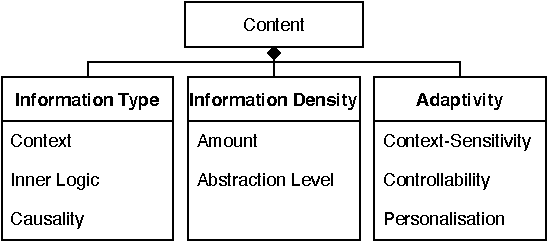
\includegraphics{contents/05_model_description/res/model_content_overview.pdf}
    \end{center}
    \caption{Übersicht über den \textit{Content} von Erklärungen}
    \label{fig:model_content_overview}
\end{figure}

\subsubsection{Inhalt}

Unter dem Punkt \textit{Content} wird definiert, mit welchen Inhalten die \textit{End User} durch Erklärungen versorgt werden \cite{nunes_systematic_2017}. Dieser ist einer von zwei Teilen des Modells, welcher sich auf die Granularität von Erklärungen bezieht. Der \textit{Content} beinhaltet nicht nur den Informationstyp (\textit{Information Type}) den das System vermittelt, sondern auch wie viel Inhalt (\textit{Information Density}). Ein weiterer Aspekt ist Anpassungsfähigkeit der Inhalte (\textit{Adaptivity}). \autoref{tab:content_of_explanations} und \autoref{fig:model_content_overview} enthalten die verschiedenen Ausprägungen dieser Aspekte zusammen mit deren Anwendungen in der Literatur, welche einen Einfluss auf die externe Qualität von Erklärungen haben.

\begin{table}[bht!]
    \begin{center}
        \begin{tabular}{p{.25\textwidth}p{.25\textwidth}p{.41\textwidth}}
            \hline
            Aspekt    & Ausprägung   & Quellen \\
            \toprule
            Information Type        & Context     & \cite{chazette2020explainability} \cite{zahedi_towards_2019}
                                                \cite{cassens_ambient_2019} \cite{zahedi_towards_2019}
                                                \cite{zolotas_towards_2019} \cite{chari_explanation_2020}
                                                \cite{nunes_systematic_2017} \cite{ribera2019can} \\
                            & Inner Logic & \cite{chazette2020explainability} \cite{sato_action-triggering_2019} 
                                                \cite{thomson_knowledge--information_2020}
                                                \cite{chari_explanation_2020} \cite{neerincx_using_2018}
                                                \cite{ribera2019can} \cite{cassens_ambient_2019} \\
                                & Causality &   \cite{chazette2020explainability} \cite{abdulrahman_belief-based_2019}
                                                \cite{yamada_evaluating_2016} \cite{sato_action-triggering_2019}
                                                \cite{zahedi_towards_2019} \cite{zahedi_towards_2019}
                                                \cite{zolotas_towards_2019} \cite{cassens_ambient_2019}
                                                \cite{thomson_knowledge--information_2020}
                                                \cite{chari_explanation_2020} \cite{neerincx_using_2018}
                                                \cite{nunes_systematic_2017}\cite{zhu_effects_2020}
                                                \cite{ribera2019can} \cite{lim_2009_assessing} 
                                                \cite{kaptein_personalised_2017} \\
            \tablerowspacing
            Information          & Amount &      \cite{ribera2019can} \cite{kouki_user_2017}
                                                \cite{hernandez-bocanegra_effects_2020} \cite{martin_developing_2019} \\
            Density              & Abstraction Level & \cite{thomson_knowledge--information_2020}
                                                \cite{hernandez-bocanegra_effects_2020} \\
            \tablerowspacing
            Adaptivity          & Context-Sensitivity & \cite{kaptein_personalised_2017} \cite{cassens_ambient_2019} \\
                                & Controllability & \cite{abdulrahman_belief-based_2019} \cite{cheng2019explaining} \\
                                & Personalization & \cite{kaptein_personalised_2017} \cite{cassens_ambient_2019}
                                                    \cite{sokol_one_2020} \cite{tintarev_designing_nodate}
                                                    \cite{sokol_explainability_2020} \\
            \toprule
        \end{tabular}
    \end{center}
    \caption{Eigenschaften einer Erklärung bezogen auf den Inhalt einer Erklärung mit in der Literatur gezeigtem Einfluss auf die externe Qualität von Erklärungen}
    \label{tab:content_of_explanations}
\end{table}

\paragraph{Information Type} Der \textit{Information Type} beschreibt die Inhalte, die \textit{End Usern} mithilfe der Erklärung übermittelt werden. Unter diesem Aspekt sind in der Literatur sehr verschiedene Ansätze zu finden, die unterschiedliche Typen definieren. Beispielsweise stellen \citeauthor{chazette_end-users_nodate} mithilfe von Fragewörtern verschiedene Informationstypen dar \cite{chazette_end-users_nodate}, während \citeauthor{rosenfeld_explainability_2019} selbige Fragewörter nutzt, um andere Inhalte zu beschreiben und weitere ergänzt. Grundsätzlich kann zwischen globalen Erklärungen, die immer gültig sind und situationsabhängigen (lokalen) Erklärungen unterschieden werden \cite{lim_2009_assessing}. Zusammen mit weiteren Arbeiten \cite{kaptein_personalised_2017, abdulrahman_belief-based_2019} wurden die verschiedenen Definitionen in drei verschiedene Informationstypen gebündelt. Diese fassen die in der Literatur am häufigsten transportierten Informationen zusammen. Allerdings bilden die drei Ausprägungen nicht alle möglichen Informationen in Erklärungen ab.

Kontextinformationen in einer Erklärung geben Auskunft über die zugrundeliegenden Daten (\textit{Context}). Dabei werden die eingehenden Informationen auf Basis derer das System Entscheidungen trifft, dem \textit{End User} dargelegt.

Eine weitere Möglichkeit ist das Erklären der Funktionsweise von Algorithmen eines Systems (\textit{Inner Logic}). Dies sind die Informationen, wie genau ein System die ihm zur Verfügung stehenden Daten verarbeitet und interpretiert.

Ein dritter Weg ist die Erklärung von Zusammenhängen zwischen den Eingaben und Ausgaben des Systems (\textit{Causality}). In einer solchen Erklärung wird den \textit{End Usern} der Grund für ein bestimmtes Systemverhalten oder eine Entscheidung erklärt. Hierbei gibt es verschiedene Optionen, Gründe zu erläutern. Eine Erklärung dieser Art kann die Information enthalten, warum ein bestimmtes Systemverhalten in einer Situation erfolgt ist. Auch kann eine Erklärung vermitteln, warum ein alternatives Verhalten oder eine alternative Ausgabe des Systems nicht erfolgt ist \cite{martin_evaluating_2021}.

\paragraph{Information Density} Die \textit{Information Density} beschreibt die Menge und die Kompaktheit an Informationen, die eine Erklärung enthält. Dabei ist einerseits wichtig, ob \textit{End Usern} alle vorliegenden Erklärungsmöglichkeiten vom System angezeigt werden (\textit{Amount}). Andererseits spielt es eine Rolle mit welchem Detailgrad die Informationen dargestellt werden (\textit{Abstraction Level}). Zum Beispiel können \textit{End Usern} wenig Informationen angezeigt werden, die nicht die vollen Details abdecken, um diese nicht zu überfordern.

\paragraph{Adaptivity} \textit{Adaptivity} definiert, wie statisch die Erklärungen in einem System sind. Eine Ausprägung ist dabei der Grad, zu dem eine Erklärung auf den aktuellen \textit{Context} angepasst ist (\textit{Context-Sensitivity}). Außerdem beinhaltet \textit{Adaptivity} die \textit{Personalisation}, welche darstellt, inwiefern Erklärungen auf den aktuellen \textit{End User} anpassbar sind, zum Beispiel an dessen Expertise. \textit{Controllability} beschreibt dabei, welchen Einfluss \textit{End User} haben, mit der Erklärung zu interagieren. Unter diesen Aspekt fällt unter anderem die Möglichkeit, dass \textit{End User} Erklärungen optional anfordern können oder sie innerhalb eines Erklärungsdialogs navigieren können.

\bigskip

An dieser Stelle kann für \textbf{RQ2} hinzugefügt werden, dass auch der \textit{Content} einer Erklärung einen großen Einfluss auf die externe Qualität von Erklärungen hat. Dies lässt sich unter anderem an der Anzahl an Autoren festmachen, die verschiedene Facetten des Einflusses durch den \textit{Content} von Erklärungen auf die Qualität untersuchen.

\subsubsection{Presentation}

Nachdem nun sowohl der \textit{Demand} als auch der an den \textit{End User} übermittelte Inhalt als zentrale \textit{Characteristics} von Erklärungen vorgestellt wurden, fehlt im Modell die Art der Präsentation der Erklärung an den \textit{End User}. Diese ist mit ihren zugehörigen Ausprägungen unter \textit{Presentation} zusammengefasst (siehe \autoref{fig:model_presentation_overview}). Sie stellt den zweiten Teil der Granularität von Erklärungen dar. Zu dem Aspekt gehören in diesem Modell für Erklärungen das Medium (\textit{Medium}), über das die Erklärung \textit{End Usern} bereitgestellt wird, der verwendete Ton (\textit{Tone}) des \textit{Explainers} (siehe \autoref{02_basics:explainability}) \cite[vgl.][]{chazette_knowledge_nodate} und die Gruppierung von Erklärungen respektive Erklärungstypen (\textit{Grouping}). \autoref{tab:presentation_of_explanations} stellt die Ausprägungen zusammen mit der Literatur, die den entsprechenden Aspekt in Bezug auf die externe Qualität von Erklärungen untersucht, dar.

\begin{figure}[t!]
    \begin{center}
        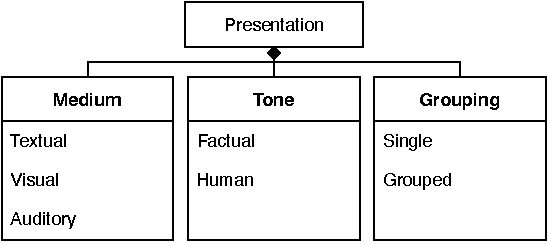
\includegraphics{contents/05_model_description/res/model_presentation_overview.pdf}
    \end{center}
    \caption{Übersicht über die \textit{Presentation} von Erklärungen}
    \label{fig:model_presentation_overview}
\end{figure}

\paragraph{Medium} Das \textit{Medium} einer Erklärung ist der Informationsträger für die \textit{Presentation} der Inhalte. Dabei können verschiedene Möglichkeiten aus dem Multimedia-Bereich verwendet werden. In der Literatur untersucht wurden Texterklärungen (\textit{Textual}), visuelle Darstellungen wie z.~B. Diagramme (\textit{Visual}) sowie auditive Erklärungen (\textit{Auditory}). Insbesondere dieser Aspekt bietet Möglichkeiten für Mischformen und Kombinationen \cite{kouki_user_2017}.

\paragraph{Tone} Der \textit{Tone} einer Erklärung bestimmt die Art, wie \textit{End Usern} der Inhalt einer Erklärung näher gebracht wird. Das Spektrum der Möglichkeiten erstreckt sich dabei vor allem zwischen sehr faktisch gehaltenen Erklärungen (\textit{Factual}) und persönlichen bzw. menschlichen Erklärungen (\textit{Human}). Ein Beispiel wäre die Bereitstellung von Erklärungen über einen persönlichen Assistenten \cite{schaffer_i_2019}.

\paragraph{Grouping} Mit dem \textit{Grouping} von Erklärungen wird bestimmt, wie viele Erklärungen \textit{End Usern} gleichzeitig beziehungsweise kombiniert präsentiert werden. Zum Beispiel können erklärende Grafiken wie Graphen mit Texterklärungen kombiniert werden. Grundsätzlich gibt es dabei die Möglichkeiten eine Erklärung zu einem Zeitpunkt anzuzeigen (\textit{Single}) oder mehrere Erklärungen bzw. Erklärungstypen zu gruppieren (\textit{Grouped}). Bei letzterem können entweder Erklärungen mit verschiedener \textit{Presentation} aber dem gleichen \textit{Content} kombiniert werden \cite{kouki_user_2017} oder mehrere einzelne Erklärungen zusammen dargestellt werden \cite{balog_measuring_2020}.

\bigskip

Als letzter Teil der Antwort auf \textbf{RQ2} kann die \textit{Presentation} mit den dazugehörigen Aspekten als Eigenschaft von Erklärungen mit einem Einfluss auf die externe Qualität von Erklärungen ergänzt werden.

\newpage

\begin{table}[htb!]
    \begin{center}
        \begin{tabular}{p{.25\textwidth}p{.25\textwidth}p{.41\textwidth}}
            \hline
            Aspekt     & Ausprägung & Quellen \\
            \toprule
            Medium              & Textual  &    \cite{sokol_explainability_2020} \cite{balog_measuring_2020}
                                                \cite{tintarev_designing_nodate} \cite{sato_action-triggering_2019}
                                                \cite{eiband_impact_2019} \cite{eiband_impact_2019}
                                                \cite{abdulrahman_belief-based_2019} \cite{cassens_ambient_2019}
                                                \cite{nunes_systematic_2017} \\
                                & Visual    &   \cite{sokol_explainability_2020} \cite{sato_action-triggering_2019} 
                                                \cite{mucha_interfaces_2021} \cite{abdulrahman_belief-based_2019}
                                                \cite{nunes_systematic_2017} \cite{schrills_color_2020} \\
                                & Auditory     &   \cite{wiegand2019drive} \cite{nunes_systematic_2017}
                                                \cite{wang_is_2018} \\
            \tablerowspacing
            Tone                & Factual   &   \cite{eiband_impact_2019} \cite{abdulrahman_belief-based_2019}
                                                \cite{kunkel_let_2019} \cite{neerincx_using_2018} \\
                                & Human     &   \cite{abdulrahman_belief-based_2019} \cite{kunkel_let_2019}
                                                \cite{weitz_you_2019} \cite{zahedi_towards_2019}
                                                \cite{neerincx_using_2018} \\
            \tablerowspacing
            Grouping            & Single    &   \cite{nunes_systematic_2017} \cite{balog_measuring_2020}
                                                \cite{sato_action-triggering_2019} \cite{eiband_impact_2019}
                                                \cite{abdulrahman_belief-based_2019} \\
                                & Grouped   &   \cite{nunes_systematic_2017} \cite{balog_measuring_2020}
                                                \cite{tintarev_designing_nodate}  \\
            \toprule
        \end{tabular}
    \end{center}
    \caption{Verschiedene Übermittlungsmöglichkeiten für Erklärungen an den \textit{End User}, die in der Literatur einen Effekt auf die externe Qualität von Erklärungen gezeigt haben}
    \label{tab:presentation_of_explanations}
\end{table}

\noindent\fbox{
    \parbox{0.964\textwidth}{
        \smallskip
        \textbf{RQ2} Welche Eigenschaften von Erklärungen haben einen Einfluss auf die externe Qualität eines erklärbaren Systems?
        \smallskip
    }
}

\smallskip

Der in diesem Abschnitt vorgestellte Teil des Modells für Erklärungen (\textit{Characteristics}) beinhaltet die Antwort auf die zweite Forschungsfrage. Dabei sind explizit die Eigenschaften \textit{Demand}, \textit{Content} und \textit{Presentation} mit einem Einfluss auf die externe Qualität von Erklärungen zu benennen. Die genauen Ausprägungen dieser Eigenschaften werden als Unterpunkte der jeweiligen Aspekte im Modell enthalten. Die Ergebnisse, die in dem Modell zusammengefasst sind, entspringen dabei der Evaluation von Erklärungen mit verschiedenen Eigenschaften in der Literatur.

\subsection{Evaluation}
\label{sec:model_evaluation_description}

Die Metriken und die Vorgehensweise, die für die \textit{Evaluation} ausgewählt wird, hängt folglich sehr eng mit den zuvor festgelegten \textit{Objectives} zusammen.

\paragraph{Target} Zunächst muss bei der Evaluation geklärt werden, was der Prüfgegenstand ist. Dabei gibt es vor allem zwei große Möglichkeiten im Kontext der Erklärbarkeit. Entweder werden die integrierten Erklärungen an sich evaluiert und die Studienteilnehmer darauf explizit angesprochen oder es werden die Auswirkungen auf verschiedene System-Metriken ausgewertet. Auch eine Kombination ist möglich.

\paragraph{Strategy} Beim Festlegen der \textit{Strategy} der Evaluation gibt es verschiedene Möglichkeiten, die unter anderem vom \textit{Context} abhängen. Je nachdem, welche Ergebnisse die Stakeholder, die Erklärungen in ein System integrieren möchten, benötigen, muss die Evaluation kontrollierter oder weniger kontrolliert sein \cite[vgl.][]{wohlin2012experimentation}.

\paragraph{Metrics} \textit{Metrics} sind klar definierte Messungen, die durchgeführt werden, um die zuvor festglegten \textit{Objectives} zu überprüfen.

Die Literaturrecherche hat wie bereits \cite{nunes_systematic_2017} nur empirische Studien zur Evaluation von Erklärungen gefunden.

Entsprechend \cite{wohlin2012experimentation} habe ich die verschiedenen Evaluationsmethoden in \textit{Qualitaative Research} und \textit{Quantitative Research} gegliedert.

\begin{table}[htb!]
    \begin{center}
        \begin{tabular}{|p{.3\textwidth}|p{.3\textwidth}|p{.3\textwidth}|}
            \hline
            \textbf{Evaluationstyp} & \textbf{Empirische Strategie} & \textbf{Quellen} \\ \hline
            Qualitativ  & Subjective Perception Questionaire &  \cite{balog_measuring_2020} \cite{sato_context_nodate}
                                                                \cite{waa_evaluating_2021} \cite{eiband_impact_2019}  \cite{kouki_user_2017} \cite{tsai_evaluating_2019}
                                                                \cite{hernandez-bocanegra_effects_2020}
                                                                \cite{zahedi_towards_2019} \cite{tsai_effects_2020} 
                                                                \cite{ribera2019can} \\
                        & Acceptance                        & \cite{tintarev_designing_nodate}
                                                            \cite{hernandez-bocanegra_effects_2020}
                                                            \cite{kunkel_let_2019} \\
                        & Think aloud                       & \cite{wiegand_id_2020} \cite{yamada_evaluating_2016} \\
                        & Preference                        & \cite{kouki_user_2017} \cite{mucha_interfaces_2021} 
                                                            \cite{abdulrahman_belief-based_2019} 
                                                            \cite{waa_evaluating_2021} \cite{wiegand_id_2020} ,
                                                            \cite{stange_effects_2021} \cite{kaptein_personalised_2017} \\
                        & Mental Model Understanding        & \cite{gunning2019darpa} \\
                        & Cognitive Workload                & \cite{wiegand2019drive, wiegand_id_2020} \\
            \hline
            Quantitative& Explanation exposure delta & \\
                        & Accuracy                          & \cite{tintarev_designing_nodate}
                                                            \cite{waa_evaluating_2021} \cite{mucha_interfaces_2021}
                                                            \cite{kunkel_let_2019} \cite{zolotas_towards_2019} \\
                        & Learning Rate                     & \cite{tintarev_designing_nodate} \cite{gunning2019darpa} \\
                        & Task Performance                  & \cite{waa_evaluating_2021}  \cite{mucha_interfaces_2021}  
                                                            \cite{abdulrahman_belief-based_2019} 
                                                            \cite{zolotas_towards_2019} \cite{martin_developing_2019} 
                                                            \cite{martin_evaluating_2021} \cite{gunning2019darpa} \\
            \hline
        \end{tabular}
    \end{center}
    \caption{Evaluation}
    \label{tab:evaluation_of_explanations}
\end{table}


Laut \cite{balog_measuring_2020} sind die 8 verschiedenen Ziele korreliert und müssen nicht einzeln gemessen werden. Hoch korreliert \cite{kouki_user_2017}

Cognitive Workload 

Einen vollständigen Überblick über die Qualität einer Erklärung bekommt man, wenn man Satisfaction, Scrutability und Translarency misst \cite{balog_measuring_2020}.

\glqq Importantly however, such measures often only measure one aspect of behavior. Ideally, a combination of both measurement types should be used to assess effects on both the user’s perception and behavior. In this way, a complete perspective on a construct can be obtained.\grqq{} (Qualitative / Quantitavie) \cite{waa_evaluating_2021}

Number of detailed looks

\subsubsection{Example Questions for questionaires}

NASA-TLX \cite{tsai_evaluating_2019}

Effectiveness helps me to determine how well I will like this movie does not help me make a decision about this item Efficiency helps me to decide faster if I will like this movie does not save me time Persuasiveness makes me want to watch this movie fails to make this item appeal to me Satisfaction would improve how easy it is to pick a recommendation does not satisfy me Scrutability would allow me to give feedback on how well my preferences have been understood would make it difficult for me to correct the reasoning behind the recommendation Transparency helps me to understand what the recommendation is based on fails to reveal the reasoning behind this recommendation Trust helps me to trust the recommendation does not seem credible \cite{balog_measuring_2020}

\cite{knijnenburg2012explaining, hernandez-bocanegra_effects_2020} have something for exact evaluation of overall explanation quality

\cite{weitz_you_2019} trusted automation questionaire

Directly based on the explatnation \cite{sato_action-triggering_2019} or other metrics 

DARPA (used by \cite{martin_evaluating_2021}) \cite{gunning2019darpa}

Domain specifc metrics. For example for explainable AI (Predictive systems) TYN (Trust-Your-Neighbours) or Meet in the Mittle (MITM) \cite{martin_evaluating_2021}

Questions for quality factors:

\subsubsection{Direkte Metriken}

Bei der direkten Messung der Qualität von Erklärungen werden in der Literatur ledig verschiedene Möglichkeiten zur subjektiven Evaluation vorgestellt.

Neben den in \autoref{sec:model_external_dependencies} vorgestellten Qualitätsaspekten, die als Qualitätsziele für die Integration von Erklärungen definiert definiert wurden, gibt es weitere Aspekte, die in der Literatur zur Messung der Qualität von Erklärungen vorgestellt wurden \cite[sato_action-triggering_2019, ], die im folgenden erläutert werden.

\paragraph{Usefulness}

\paragraph{Completeness}

\paragraph{Correctness}

Bei der Messung der direkten Messung der Erklärugnsqualität setzt die Literatur vor allem Likert-Skalen ein. Dabei handelt es sich um einen Ordinalskala mit in der Regel fünf oder sieben einzelnen Bewertungsschritten, auf denen einen Aussage bewertet wird. Die genaue Benennung der Bewertungsschritte erfolgt in der Literatur verschieden. Allerdings werden durchweg solche mit einer inhaltlichen Übereinstimmtung zu \glqq Volle Zustimmung\grqq{}, \glqq Teilweise Zustimmung\grqq{}, \glqq Neutral\grqq{},\glqq Teilweise Ablehnung\grqq{} und \glqq Volle Ablehnung\grqq{} verwendet \cite{sato_action-triggering_2019, sato_context_nodate, wang_is_2018, hoffman_metrics_nodate}. \autoref{tab:evaluation_direct_measures_evaluation} stellt eine Übersicht von verwendeten Aussagen für die Messung der verschiedenen Aspekte dar. Aufgelistet sind nur verallgemeinerbare Aussagen und nicht einen spezifischen \textit{Context} betreffende Aussagen. In spitzen Klammer sind Platzhalter dargestellt, um die aufgelisteten Aussagen auf den eigenen \textit{Context} anzupassen.

\begin{table}
    \begin{center}
        \begin{tabular}{|p{0.25\textwidth} p{0.5\textwidth} p{0.15\textwidth}|}
            \hline
            \textbf{Qualitätsaspekt} & \textbf{Aussage} & \textbf{Quellen} \\
            \hline
            \hline
            Transparency    & & \\
            \hline
            Satisfaction    & Ich bin zufrieden mit der Erklärung, um zu verstehen, warum das System seine Entscheidung 
                                getroffen hat.
                                & \cite[vgl.][]{riveiro_thats_2021} \\
            \hline
            Transparency    & & \\
            \hline
            Persuasiveness  & Die Erklärung ist überzeugend.
                                & \cite[vgl.][]{sato_action-triggering_2019, sato_context_nodate} \\
                            & Die Erklärung weckt Interesse. 
                                & \cite[vgl.][]{sato_action-triggering_2019, sato_context_nodate} \\
            \hline
            Usefulness      & Die Erklärung ist einfach zu verstehen. 
                                & \cite[vgl.][]{sato_action-triggering_2019, sato_context_nodate} \\
                            & Die Erklärung ist nützlich bei der Erfüllung von <Aufgabe>.
                                & \cite[vgl.][]{sato_action-triggering_2019, sato_context_nodate} \\
            \hline
            Completeness    & & \\
            \hline
            Completeness    & & \\
            \hline
        \end{tabular}
    \end{center}
    \caption{}
    \label{tab:evaluation_direct_measures_evaluation}
\end{table}

\subsubsection{Indirekte Metriken}

\begin{itemize}
    \item Satisfaction: The explanations provided of how the AI-system classifies text are satisfying. \cite{riveiro_thats_2021}
    \item Completeness: The explanations provided regarding how the AI-system classifies the text seem complete
 \cite{riveiro_thats_2021}
    \item Completeness: Would you have liked for the explanations to contain additional information? If so, what type of information and when, i.e., in which situations?
 \cite{riveiro_thats_2021}
    \item Sufficient detail: The explanations provided of how the AI-system works have sufficient detail.
 \cite{riveiro_thats_2021}
    \item Understanding: From the explanations provided, I understand how the AI-system works.
 \cite{riveiro_thats_2021}
 \item Transparency: I understand the robot’s decision-making process \cite{wang_is_2018}
 \item Understandability: The explanation helps me understand how the [software, algorithm, tool] works. \cite{hoffman_metrics_nodate}
 \item Satisfaction: The explanation of how the [software, algorithm, tool] works is satisfying. \cite{hoffman_metrics_nodate}
 \item Completeness: The explanation of how the [software, algorithm, tool] works is sufficiently complete. \cite{hoffman_metrics_nodate}
 \item Helpfull: The explanation is actionable, that is, it helps me know how to use the [software, algorithm, tool] \cite{hoffman_metrics_nodate}
 \item Correctness: The explanation lets me know how accurate or reliable the [software, algorithm] is.\cite{hoffman_metrics_nodate}
 \item Trust: The explanation lets me know how trustworthy the [software, algorithm, tool] is. \cite{hoffman_metrics_nodate}
\end{itemize}


Tabelle der Metriken nach \cite{carvalho2017quality} (Ubiqutous Systems)

Trustworthiness: \cite{schrills_color_2020}

(FOST Scale: Facets of System Trustworthiness)
Please indicate to what extent you agree with the following statements 01 The system’s classification is reliable 02 The system’s classification is precise 03 The system’s classification is traceable 04 I can trust the system’s classification 05r I cannot depend on the system’s classification 06 With the help of the visualization I am able to identify wrong mechanisms of the AI 07 I agree with the classification 08 The visualization provides a good explanation for the classification

\cite{tintarev_designing_nodate} haben Messliste gebaut.

(Task performance) \cite{martin_evaluating_2021}

Qualität von Erklärungen zu bestimmen ist nicht einfach.

\cite{tsai_effects_2020}:

Construct E: Perceived System Effectiveness • E1: Using the system is a pleasant experience. • E2: I made better choices with the recommender. • E3: I found better items using the recommender. • E4: I felt bored when using the recommender. • Construct T: Perceived Trust • T1: I am convinced by the scholar recommended to me. • T2: I am confident I will like the items recommended to me. • T3: The recommender made me more confident about my selection/decision. • T4: The recommender can be trusted. • Construct P: Perceived Transparency • P1: The provided information was sufficient for me to make a good decision. • P2: The recommender explained why the scholars were recommended to me. • P3: I understood why the scholars were recommended to me. • Construct S: Satisfaction • S1: I will use this recommender again. • S2: I will tell my friends about this recommender. S3: Overall, I am satisfied with the recommender. • S4: The recommender helped me find the ideal contacts at the conference.

Special measures like ICM for ML-Models which is tied to the input and output of the model \cite{waa_evaluating_2021, neerincx_using_2018}

Trust questions: originally by \cite{mayer1999effect} used by \cite{wang_is_2018}

Specific trust items e.g. for human-robot interaction used by \cite{zhu_effects_2020} originally developed by \cite{schaefer2013perception}

Just different Begriffe mit Likert SCale (Satisfaction / Trust / Transparency) \cite{koo_understanding_2016, koo_why_2015} Behavioral is again domain specific

3 Types of Evaluation according to \cite{ribera2019can, doshi2017towards}: (1) applicationgrounded evaluation with real humans and real tasks; (2) human-grounded evaluation with real humans but simplified tasks; and (3) functionally-grounded evaluation without humans and proxy tasks; all of them always inspired by real tasks and real humans’ observations.

 \cite{tintarev2007survey}:
 
 Transparency: Qualitytive: Does the User understand the system Quantitative: correctness, completion time
 
 Scrutability: Hard to measure due to many confoundings
 
 Trust: Questionaires, Loyalty: Number of Logins, usesages (S. M. McNee, S. K. Lam, J. A. Konstan, and J. Riedl. Interfaces for eliciting new user preferences in recommender systems. User Modeling, pages pp. 178–187, 2003.)
 
 Persuasiveness: Questionaires + Domain-Specific Performance metrics
 
 Effectiveness: accuracy measures (Domain-Specific) 
 
 Efficiency: Task completion time, Number of times an explanation is called
 
 Satisfaction: User preference (Differentiate explanation and system), number of usability problems
 
 Wichtig ist auch das Messen von anderen Qualitätsaspekten, die nicht 

\section{Abhängigkeiten}
\label{sec:model_proved_relations}

\cite{international2011iso} definiert ein Konzept, um Zusammenhänge zwischen Charakteristiken eines Systems und Qualitätsaspekten zu definieren. Anwendung findet dies unter Anderem bei \cite{carvalho2020developers}. Das Konzept beschreibt, dass einzelne Eigenschaften von Softwaresystemen einen positiven (\textcolor{green}{helps}), negativen (\textcolor{red}{hurts}) oder neutralen Effekt auf Qualitätsaspekte haben kann. Diese können entweder generell gelten oder unter bestimmten Bedingungen (Kontexten) zutreffen.

\subsection*{Demand}

\subsubsection*{Positiv}

Eine Erklärung die den Kontext des Systemverhaltens wiederspiegelt wirkt sich positiv auf die Persuasiveness und die Usefullness einer Erklärung aus. Bewiesen ist dies nur für Recommender Systeme \cite{sato_action-triggering_2019, abdulrahman_belief-based_2019}

Eine Erklärung, die darstellt, warum eine Alternative nicht genommen wurde, wird besser verstanden als eine, welche die aktuelle Entscheidung erklärt. \cite{schrills_color_2020}

(2) Rational explanations are only effective on users that report being very unfamiliar with a task – regardless of their actual competency level. \cite{schaffer_i_2019}

Das proaktive Präsentieren von Erklärungen, wenn diese einen geringen Inhalt haben wirkt sich positiv auf die Usability aus.

Das Anzeigen von Erklärungen vor einem Event hat einen positiveren Einfluss auf Trust als das Anzeigen danach. \cite{haspiel_explanations_2018}

Proaktive Erklärungen in unvorhersehbaren Situation, erhöhen das Vertrauen \cite{zhu_effects_2020}

Das anzeigen von Erklärungen bei sicherheitsrelevanten Systemfunktionen hat einen positiven Einfluss auf satisfaction und trust. \cite{wiegand2019drive}

Nutzer wollen immer Zugriffsmöglichkeiten auf erklärungen \cite{chazette_end-users_nodate}

\subsubsection*{Negativ}

(3) There is a danger in showing explanations to self-confident users in that situation awareness might be negatively impacted – this can be mitigated by requiring interaction with an agent. \cite{schaffer_i_2019}

\subsubsection*{Beides}

Der Zusammenhang zwischen dem Grad der Systembeeinflussung durch den Nutzer und dem Erklärungsbedarf ist antiproportional. Umso mehr mehr Kontrolle der Nutzer über ein System erhält, umso weniger Erklärungsbedarf hat dieser \cite{rosenfeld_explainability_2019}.

Wenn der Nutzer generell ein hohes Vertrauen in ein System hat, dann benötigt dieser keine Erklärungen, um dieses herzustellen. \cite{rosenfeld_explainability_2019, doshi2017towards}

Die User Satisfaction kann leiden, wenn die Nutzer das System bereits gut kennen, wenn eine Erklärung angezeigt wird.

\subsection*{Granularität}

\subsubsection*{Positiv}

Hybride Stile (Typ + Inhalt) haben den größten positiven Einfluss auf die Usability und Persuasiveness eines Recommender Systems im Gegensatz zu einzeln ausgewählten Stilen. \cite{sato_action-triggering_2019, kunkel_let_2019, sato_action-triggering_2019, schrills_color_2020, lim_2009_assessing}

Das Präsentieren von Erklärungen durch Agenten hat einen positiven Einfluss auf Trust in intelligenten System \cite{weitz_you_2019}.

Das Geben von Kontextinformationen beeinflusst Usefullness und Persuasivness am positivsten im Vergleich zu keinen oder Inhaltsbasierten erklärungen \cite{sato_action-triggering_2019}

Non-experts prefer belief-based explanations and experts perefer goal-based \cite{kaptein_personalised_2017}, hypotthesis (The letter is proved by \cite{martin_evaluating_2021})

Counterfactual (Why not) ist better bei Alternativen \cite{martin_evaluating_2021, schrills_color_2020}  \cite{neerincx_using_2018} \cite{schrills_color_2020} (Small significant effect), \cite{lim_2009_assessing} sagt, dass das nicht trivial ist.

Bessere Transparenz durch erklärungen, wenn der Nutzer generell ein geringes Vertrauen in Technologie oder höhere Privacy concerns im Allgemeinen hat. \cite{tsai_effects_2020}

Personalisierte Erklärungen erhöhen die Transparenz \cite{sokol_one_2020, wiegand2019drive}

Wenn der User mit dem Output des Systems übereinstimmt, dann erhöht dies den Trust in das System. \cite{schrills_color_2020}

Einfache Erklärungen führen zu einer höheren Akzeptanz der Erklärungen und zu höherer Nutzerzufrienenheit \cite{hleg2019policy, sovrano_modelling_2020}

Interactive Erklären erhöhen das Verständnis \cite{cheng2019explaining}

Context und Causality sind die am meisten angefragten Informationen \cite{chazette_end-users_nodate}

Die Anzahl der Paper bestätigt das Ergebnis von \cite{chazette_end-users_nodate}, dass die Reihenfolge der Häufigkeiten mit der die Inhalte untersucht wurden so ist. (How ist unnötig.)

\subsubsection*{Negativ}

Wenn User nicht mit der Ausgabe des Systems übereinstimmen, dann 

lack of completeness \cite{chazette_end-users_nodate} -> Kann durch interactivity umgangen werden

Wenn ein Assistent, der für Erklärungen genutzt wird zu lächerlich gestaltet ist, kann dies zu einem vertrauensverlust führen. \cite{wang_is_2018}

Behaviour information might have a negativ effect on satisfaction due to redundance with the system behaviour it self und kann sogar zu schlechterer Nutzer Performance führen. \cite{koo_why_2015}

Recommender Systems Repetetive Erklärungen \glqq langweilig\grqq{}

Wenn der Nutzer durch eine Erklärung zu sehr davon Überzeugt ist, das System verstanden haben, kann dies einen negativen Impact auf die Effectivity haben, da er Fehler des Systems nicht erkennt. (Cognitive bias) \cite{kohl_explainability_2019}

why information is good for transparency \cite{chazette2020explainability}

\subsubsection*{Neutral}

Die Richtigkeit einer Erklärung hat keinen Einfluss auf das Vertrauen des Endnutzers in das System, wenn das Verhalten des Systems mit dem Mentalen Modells des Nutzers übereinstimmt. \cite{eiband_impact_2019, riveiro_thats_2021}

Es gibt keinen Zusammen zwischen dem Ziel mit dem die Erklärung verfasst wurde und dem Effekt, der sich auf die verschiedenen Ziele messen lässt, bei einer Formulierung durch den Menschen. \cite{balog_measuring_2020}.

Bei der Inhaltlichen Abfrage steht \cite{zahedi_towards_2019} gegen chazeete (Genaues paper suchen). Folglich scheint der Inhaltstyp keinen großen Einfluss auf die Erklärung zu haben. Wenn allerdings die 

Transparency might not increase the Trust solely. The explanation has to fit it's goal \cite{wiegand2019drive}

User haben höhere Anfroderungen and why erklärungen, weswegen diese öfter als nicht hilfreich gekennzwichnet werden als How-Fragen. \cite{lim_2009_assessing}

There ist no prove up to now that interactions increase trust \cite{cheng2019explaining}
-------------------------------------------------------------------

Scrutability and Trust are related: Zu viel Trust -> Der User erkennt nicht mehr, wenn das System falsch ist. \cite{gunning2019darpa}

Für die verschiedenen Systemkontexte gibt es weitere Zusammenhänge, die eine Rolle spielen. Als Beispiele wäre hier zum Beispiel zu nennen, dass User Erklärungen im AI-Kontext... Im Recommender System Kontext wäre das...

Da das Ziel dieser Arbeit allerdings ein allgemeiner Überblick über Erklärbarkeit mit seinen Zusammenhängen und Eigenschaften von Erklärungen geben soll, werden diese an dieser Stelle ausgeklammert.

\cite{martin_evaluating_2021}: For engineers, it is about whether the explanation follows their reasoning, while desk-based agents are more concerned with whether it supports their work.

Eine Übersicht mit Arbeiten vor 2015, die im Kontext von Empfehlungssystemen einen Effekte auf eines der in \autoref{tab:quality_aspects_of_explanation} aufgelisteten Ziele hat, kann in der Arbeit von \citeauthor{nunes_systematic_2017} gefunden werden \cite{nunes_systematic_2017}.

Usability beschreibt die Qualität einer Erklärung im Bezug auf die Interaktion und die Darstellung der Inhalte \cite{chazette_end-users_nodate}. Informativeness ist dierekt bezogen auf den Inhalt der Erklärung \cite{chazette_end-users_nodate}. Direkt messbar an der Erklärung selbst.

\section{Design Empfehlungen}
\label{sec:model_design_implications}

\cite{carvalho2020developers} Nutzt einen Katalog, der die Genauen Zusammenhänge darstellt.

kontext ist sehr wichtig! \cite{sato_context_nodate}

Es sollte darauf geachtet werden, dass vor allem die wahrgenommene Performanz des Systems erhöht wird \cite{riveiro_thats_2021}

should get explanation if possible \cite{wiegand_id_2020}

Indication of system confidence \cite{wiegand_id_2020, golledge1999wayfinding}

Display context informaiton \cite{wiegand_id_2020}

\cite{weitz_you_2019} proposes to use user triggered explanations

– Low-level explanations methods allow the user to visualise key information that provide insight to system decision-making and support interpretation. \cite{martin_evaluating_2021}

– High-level explanation methods augment one or more low-level explanations with contextual information to enable more comprehensive explanation. \cite{martin_evaluating_2021}

- Beim Design einer Erklärung muss genau darauf geachtet werden, welche Kontextinformationen den Nutzer wirklich interessieren. (Beispielsweise im Kontext von AI welche Features) \cite{rjoob_towards_2021}

Umso einfacher und kürzer eine Erklärung ist, umso früher kann sie präsentiert werden. \cite{hleg2019policy, sovrano_modelling_2020}

\glqq Not only should the developers consider the quality, form, and granularity of the explanations, but also the dynamic learning process of the users \grqq{} \cite{wang_integration_2020}
